\chapter{Introducción}
%%---------------------------------------------------------

\section{Objetivos} El objetivo principal del trabajo es modernizar las herramientas
de Linked Data Geográfico desarrolladas por el Grupo de Ingeniería Ontológica. En el OEG se ha venido
tradicionalmente trabajando con el Instituto Geográfico Nacional para la exportación de algunos de sus datos
geográficos a formato Linked Data. Un ejemplo se puede encontrar en la web del Instituto Geográfico Nacional.
\cite{ign}

Desde que se publicó ``A sustainable process and toolbox for geographical linked data generation and publication:
a case study with BTN100'' en 2019\cite{toolbox}, GeoKettle ha dejado de estar soportado. La pagina oficial y de documentación
ya no están disponibles. Algunas funcionalidades de GeoKettle se integraron en PDI directamente y otras
desaparecieron. Actualmente, el soporte GIS de Pentaho está dentro de PDI Spoon y además hay algunas
funcionalidades más en el plugin llamado pentaho-gis-plugins\cite{gis-plugins}. 

Por otro lado, recientemente, el Open Geospatial Consortium ha publicado el formato GeoPackage, que tiene el
objetivo de convertirse en un estándar para la representación de datos geográficos. El siguiente objetivo de este
trabajo es el de dar soporte GeoPackage para las herramientas normalmente utilizadas para este tipo de tareas.
Ya que el 3 de abril de 2021 pentaho-gis-plugins añadió soporte geopackage a su plugin, parte del trabajo está
hecho.

En resumen:
\begin{enumerate} 
    \item Replicar la funcionalidad y las transformaciones de GeoKettle + TripleGeo en la nueva suite PDI. 
    \item Dar soporte GeoPackage a la herramienta GeoKettle y su plugin para transformar a RDF. 
    \item Realizar un procesado completo de todos los datos del IGN para generar este tipo de formato. 
\end{enumerate}

\section{Estado del Arte}

\subsection{GIS} Los sistemas de información geográfica son herramientas que permiten almacenar y analizar datos
geoespaciales. Los sistemas digitales actuales permiten realizar consultas interactivas, añadir entradas a las
bases de datos y visualizarlos de manera intuitiva. La información geográfica se puede aplicar a todo tipo de
áreas, entre las que se encuentran la ingeniería, transporte, telecomunicación, economía, sociologia... Debido a
la gran importancia tanto en el sector público como el privado\cite{gis-standards}, los estándares abiertos
cobran importancia por estar disponibles al público, no tener que pagar licencias y ser consensuados por
organizaciones de estándares internacionales. Entre ellas se encuentra el Open Geospatial Consortium(OEG) que se creó
en 1994 y agrupa a 521 (en marzo de 2021) miembros de organizaciones públicas y privadas.\cite{ogc-members}
El OGC trabaja junto con las principales organizaciones de estándares de su ámbito (ISO/TC 211, W3C,
IETF...) \cite{ogc-whitepaper}

Existen diversos formatos de fichero GIS, divididos en \textbf{raster} y \textbf{vector}. La diferencia es
equivalente a la que existe entre imágenes con resolución limitada por el número de píxeles (raster) y las 
imágenes vectoriales formadas por puntos, líneas y polígonos; con resoluciones infinitas. Cada tipo de formato
tiene sus ventajas y desventajas y la elección dependerá del caso de uso. Existen varios formatos vectoriales
pero para este trabajo sólo se se considerarán el formato \textit{shapefile} y el \textit{GeoPackage} para cumplir
los objetivos.

\begin{figure}[H]
    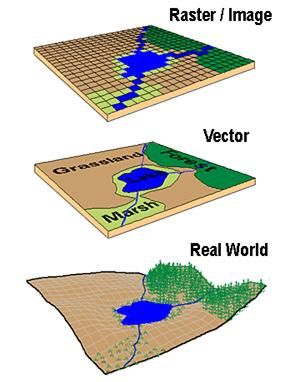
\includegraphics[width=0.4\textwidth]{images/vector-raster.jpg}
    \centering
    \caption{Representación del terreno mediante vectores y raster}
    \label{fig:vector-raster}
\end{figure}

\subsubsection{Shapefile} El formato ESRI Shapefile (SHP) es un formato de archivo de datos espaciales vectorial
desarrollado por la compañía ESRI a principios de la década de 1990. A pesar de ser propietario, la
especificación es abierta, y se considera un estandar de facto. Debido a su popularidad, goza de grán
compatibilidad con sig. Gracias al uso de un fichero índice, se obtiene una velocidad de lectura alta, y su
eficiencia de tamaño produce archivos relativamente pequeños.

Sin embargo, tiene varias desventajas, algunas derivadas del uso del estándar dBase \cite{shapefile-specs}
\cite{shapefile-no}: 

\begin{enumerate} 
    \item No tiene definición de sistema de referencia de coordenadas \footnote{Un sistema de
            coordenadas es un sistema de referencia que se utiliza para representar la ubicación de entidades
            geográficas, imágenes y observaciones (como las localizaciones GPS) dentro de un marco geográfico
            común. Los sistemas de coordenadas permiten a los datasets geográficos utilizar ubicaciones comunes
            para la integración de datasets. \cite{coordenadas}} 
        , se puede usar uno pero no es parte estándar de la especificación.     
    \item Se reparte en múltiples ficheros: es incómodo y lleva a errores al compartirlos.
    \item Los nombres de atributos están limitados a 10 caracteres ASCII 
    \item El número máximo de campos de atributo es 255.  
    \item Solo admite float, integer, date y text con un máximo de 254 caracteres.  
    \item No se puede especificar conjunto de caracteres de la BBDD.  
    \item El tamaño está limitado a 4GB.  
    \item No admite valores NULL 
    \item No hay forma de describir las relaciones topológicas en el formato.  
    \item Solamente puede almacenar una geometría por archivo.  
    \item Utiliza una estructura de datos de tabla plana, sin jerarquías, relaciones ni estructura en árbol.  
    \item El soporte 3D es muy limitado.  
\end{enumerate}

\subsubsection{GeoPackage}
GeoPackage es un formato GIS implementado en SQLite publicado por el OEG en 2014. \cite{geopackage-spec}
    
El formato geopackage tiene las siguientes ventajas \cite{shapefile-no}:
\begin{itemize}

    \item Es abierto, no propietario, basado en estándares, independiente de plataformas,
        portable y compacto.

    \item Gracias a SQLite puede almacenar datos grandes (hasta 140TB)\cite{sqlite-limits} y los atributos de
        las geometrías pueden contentener nombres muy largos.

    \item Dispone de índices espaciales basados en R-trees \cite{rtree} que incrementan la velocidad de búsquedas
        espaciales y su visualización en los SIG de escritorio.
       
    \item Todo el contenido se almacena en un único archivo .gpkg que puede almacenar multitud de tipos de
        geometrías

    \item Soporta el uso directo, para acceder a los datos de GeoPackage de forma «nativa» sin traducciones de
        formato intermedio.

    \item GeoPackage es soportado por GDAL\cite{gdal}, la librería de conversión de datos utilizada por multitud
        de programas GIS (incluído GeoKettle), y los principales programas GIS.
\end{itemize}


\subsection{Datos enlazados}
El objetivo de los datos enlazados es utilizar la web como una única base de datos global. Tim Berners Lee,
creador de la World Wide Web, quien acuñó el término linked data\cite{berners-lee}, definió sus 4 principios
fundamentales:

\begin{enumerate}
    \item Utilizar URIs para identificar los recursos publicados en la Web.
    \item Utilizar URIs HTTP para que las personas puedan consultar esos recursos.
    \item Cuando alguien acceda a una URI, proporcionar información útil mediante estándares (RDF*, SPARQL).
    \item Incluir enlaces a otras URIs para facilitar el descubrimiento de más información relacionada.
\end{enumerate}

Los datos enlazados posibilitan la web semántica, extensión de la web tradicional en la que la información tiene
significado bien definido\cite{semantic-web} y fundamentada en:
\begin{itemize}
    \item URIs: cadena de caracteres que identifica los recursos de una red de forma unívoca.
    \item RDF: método para la descripción conceptual o modelado de la información.
    \item HTTP: protocolo de comunicación.
\end{itemize}

RDF modela información mediante triples o tripletas de sujeto-predicado-objeto. El sujeto hace referencia al
recurso y el predicado a sus rasgos o aspectos y relación entre el sujeto y el objeto. SPARQL es el lenguaje para
la consulta de grafos RDF.

\subsection{Portales de Datos abiertos}

Los datos abiertos parten de la idea de que los datos deberían estar disponibles de forma libre para todo el
mundo, libre de derechos de autor, patentes o de otros mecanismos de control. Los portales de datos abiertos
proporcionan una manera sencilla de buscar y obtener estos datos. Los datos pueden tener cualquier procedencia,
pero han cobrado especial importancia los datos ligados a las políticas de Gobierno abierto, que persigue que los
datos y la información, especialmente las que poseen las administraciones públicas, se publiquen de forma
abierta. \cite{datos-madrid}

El tercer objetivo de este trabajo se centra en realizar un procesado completo de todos los datos del IGN.
\textit{datos.ign.es} es una iniciativa del Instituto Geográfico Nacional (IGN) para la generación de la información
semántica de sus recursos\cite{datos-ign}. Actualmente el dataset disponible es la Base Topográfica Nacional
1:100.000 (BTN100), un catálogo de datos geográficos agrupados por temáticas.

\subsection{Map4RDF}

Map4rdf es una herramienta para la navegación y visualización de datasets RDF con información geoespacial
mediante facetas\cite{map4rdf-paper}. Algunos ejemplos de las facetas y sus contenidos que permiten clasificar los elementos del
BTN100:

\begin{itemize}
    \item Altimetria: Cerro, Cordillera, Montaña...
    \item Hidrografía: Bahía, Cabo, Playa...
    \item Transporte: Aeropuerto, Calle, Faro...
    \item ...
\end{itemize}

El funcionamiento de Map4rdf es el siguiente:
\begin{enumerate}

    \item El componente \textit{DAO} \footnote{Data Acces Object: propociona una interfaz abstracta a una base de
        datos.} se conecta a una \textit{triplestore} \footnote{Triplestore: base de datos de tripletas} mediante
        el \textit{endpoint SPARQL} \footnote{SPARQL endpoint: url capaz de recibir y procesar peticiones del
        protocolo SPARQL} para responder a las consultas de facetas. 

    \item La interfaz de navegación facetada obtiene la lista de facetas y las visualiza. 

    \item El usuario selecciona una faceta y el componente DAO realiza una consulta en el
        triplestore mediante el endpoint SPARQL para recuperarlas la información pedida.

    \item La interfaz recibe toda esta información y la visualiza en el mapa.

\end{enumerate}

\begin{figure}[H]
    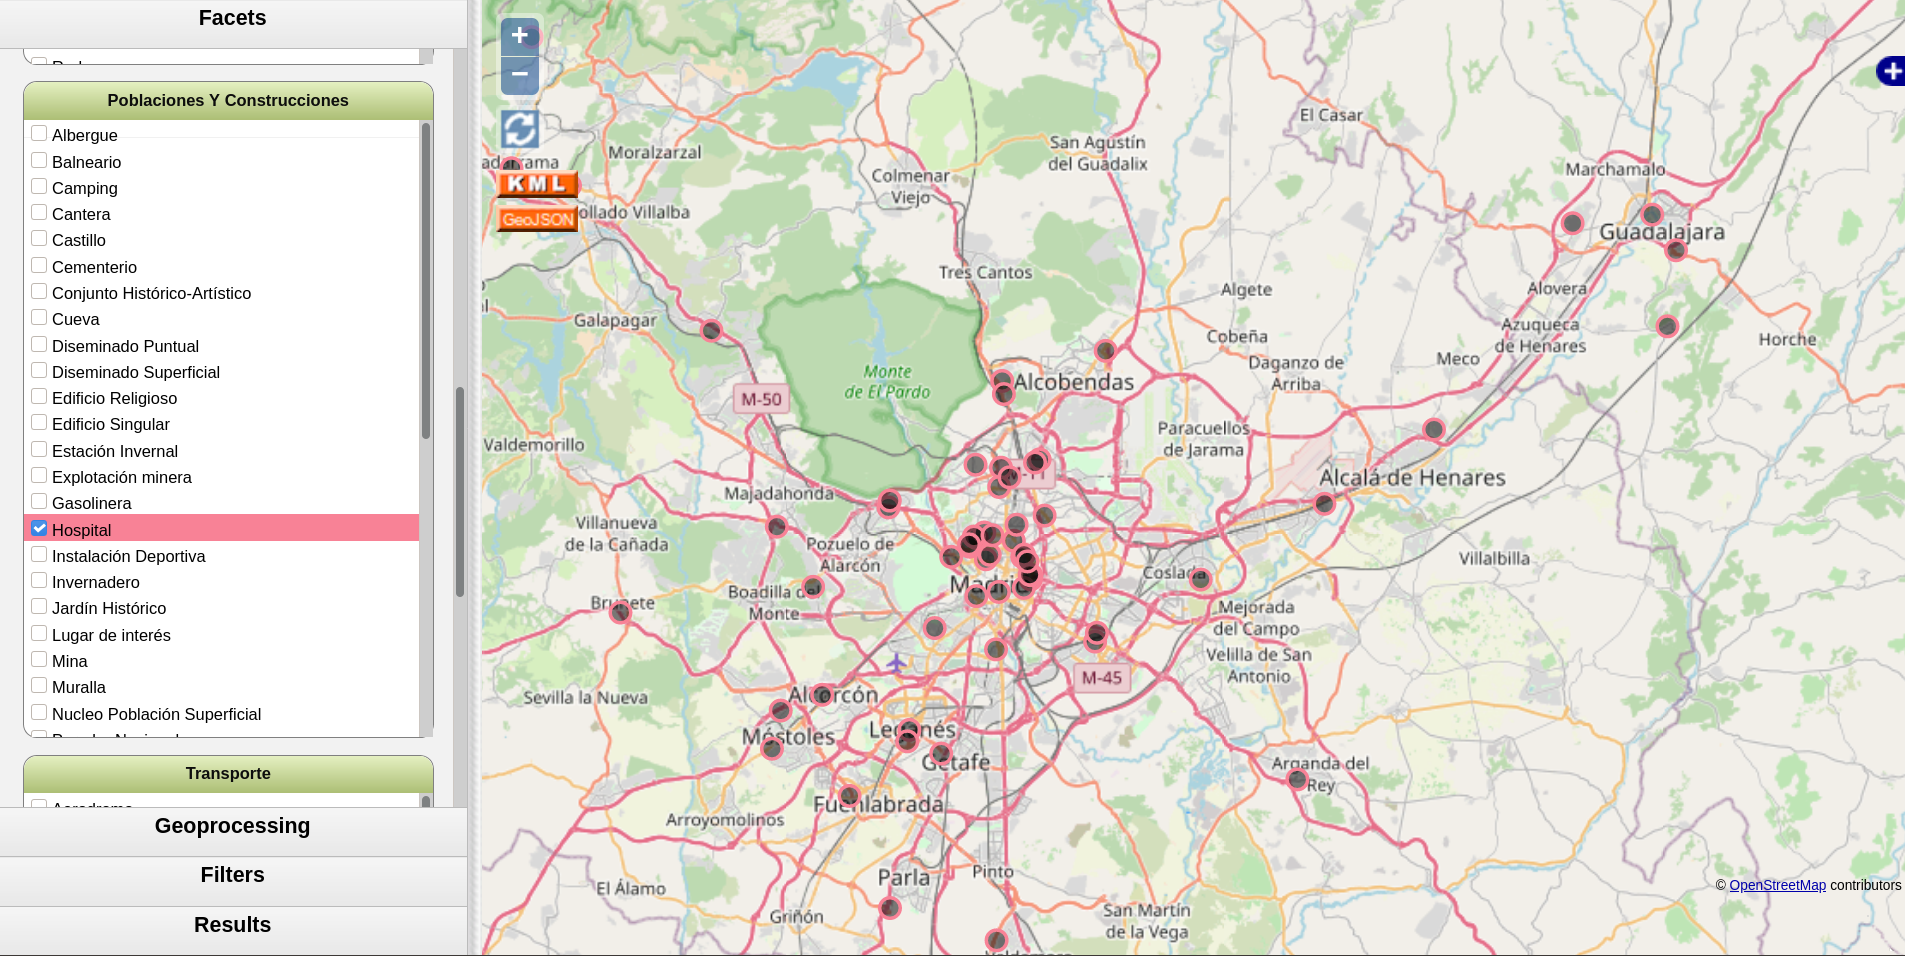
\includegraphics[width=\textwidth]{images/map4rdf.png}
    \centering
    \caption{http://certidatos.ign.es/map/ que implementa Map4Rdf}
    \label{fig:map4rdf}
\end{figure}


\subsection{GeoKettle}

GeoKettle es una (antigua) versión de Pentaho Data Integration (Kettle)\cite{pentaho} con capacidad de tratamiento de datos
espaciales. Es una potente herramienta ETL: extracción, transformación y carga orientada al uso de metadatos y
con funcionalidades espaciales dedicada a la integración de diversos orígenes de datos para la construcción y/o
actualización de bases de datos espaciales y almacenes de datos espaciales. \cite{geokettle-osg}

TripleGeo es un plugin para GeoKettle que transforma datos geoespaciales en tripletas RDF siguiendo el standar
GeoSPARQL \cite{triplegeo}

\begin{figure}[H]
    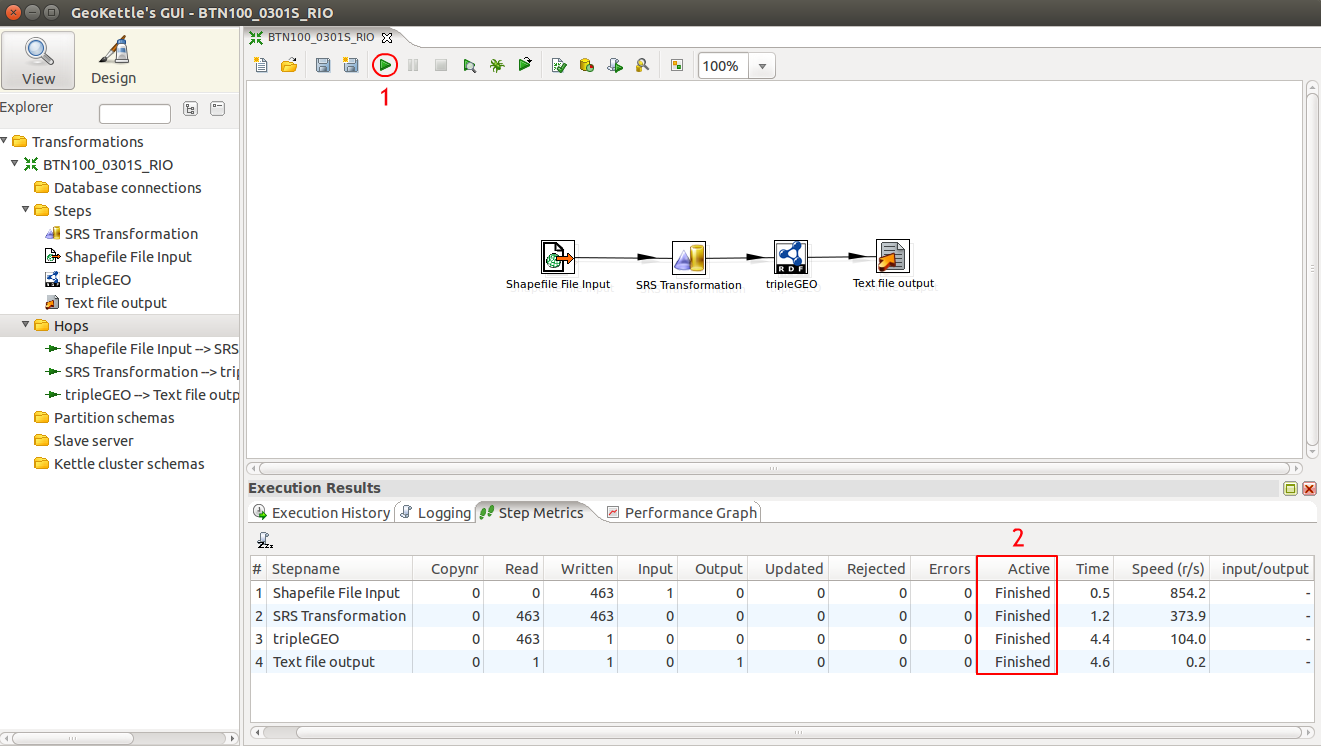
\includegraphics[width=\textwidth]{images/kettle.png}
    \centering
    \caption{TripleGeoKettle en funcionamiento, TripleGeoKettle wiki}
    \label{fig:kettle}
\end{figure}

\section{Pentaho Data Integration Spoon}

PDI Spoon\cite{pdi-spoon} es la herramienta que reemplaza a GEOKettle. La GUI, el funcionamiento y el SDK para desarrollar
plugins es parecido. Sin embargo, en cuanto al desarrollo de plugins, cambia la manera de gestionar las
dependencias, las cabeceras de algunas interfaces que se deben implementar, los iconos, metadatos, estructura de
carpetas...

\subsection{Pentaho GIS Plugins}

Es un plugin desarrollado por Atol Conseils et Développements\cite{atol} para PDI9. Proporciona parte de la funcionalidad
GIS que tenia GEOKettle. fig.\ref{fig:gis-plugins} 

\begin{figure}[H]
    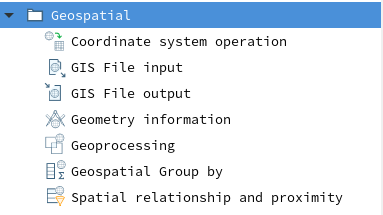
\includegraphics[width=0.6\textwidth]{images/gis-plugins.png}
    \centering
    \caption{Steps incluidos en gis-plugins}
    \label{fig:gis-plugins}
\end{figure}


\subsection{Apache Ant}

Apache Ant\cite{apache-ant} es una libreria Java y herramienta de línea de comandos para construir aplicaciones java (compilar,
ensamblar y ejecutarlas). Los scripts de configuración se escriben en formato XML y son muy flexibles.

\subsection{Apache Maven}

Apache Maven \cite{apache-maven} es una herramienta de gestión de proyectos y dependencias. Está basado en el
concepto Project Object Model (POM). Maven es capaz de construir las aplicaciones, descargar las dependencias y
gestionarlas, ejecutar tests, crear documentación...

El fichero principal, pom.xml detalla la configuración. Se pueden incluir repositorios externos y dependencias.
Maven se encarga de descargar las dependencias y sus subdependencias desde los repositorios para no tener que
hacerlo a mano.

%%---------------------------------------------------------
